\chapter{Hardware Design}

\section{Overview}

The NexusFlow hardware platform is built around the ESP32 DevKit V1 microcontroller, complemented by relay modules for device control, touch sensors for physical interaction, and environmental sensors for ambient monitoring. This chapter details component selection, circuit design, and GPIO configuration.

\section{Component Specifications}

\subsection{ESP32 DevKit V1}

\noindent
\begin{minipage}{0.4\textwidth}
\centering
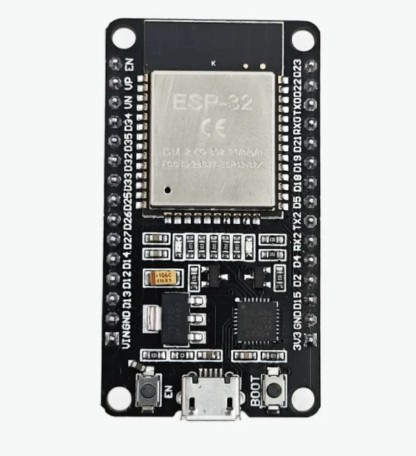
\includegraphics[width=\textwidth]{images/hardware/esp32.jpg}
\captionof{figure}{ESP32 DevKit V1 Microcontroller}
\label{fig:esp32}
\end{minipage}
\hfill
\begin{minipage}{0.55\textwidth}
\textbf{Key Specifications:}
\begin{itemize}
    \item \textbf{Processor:} Dual-core Xtensa 32-bit LX6 @ 240 MHz
    \item \textbf{RAM:} 320 KB SRAM, 4 MB Flash
    \item \textbf{Connectivity:} WiFi (802.11 b/g/n), Bluetooth 4.2 (BLE)
    \item \textbf{GPIO Pins:} 34 total (25 usable on DevKit V1)
    \item \textbf{ADC Channels:} 12-bit resolution, 8 channels
    \item \textbf{I2C/SPI:} Full support for sensor communication
    \item \textbf{Power:} 5V USB input, 3.3V internal regulation
\end{itemize}
\end{minipage}

\vspace{0.4cm}
\noindent \textbf{Rationale:} The ESP32 provides an excellent balance of processing power, wireless capabilities, GPIO availability, and cost, making it ideal for IoT applications requiring both BLE provisioning and WiFi connectivity.

\subsection{Relay Module (SRD-05VDC-SL-C)}

\noindent
\begin{minipage}{0.4\textwidth}
\centering
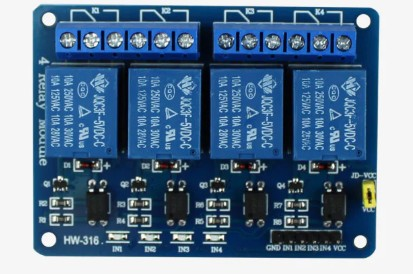
\includegraphics[width=\textwidth]{images/hardware/relay.jpg}
\captionof{figure}{5V Relay Module with Active-LOW Control}
\label{fig:relay}
\end{minipage}
\hfill
\begin{minipage}{0.55\textwidth}
\textbf{Specifications:}
\begin{itemize}
    \item \textbf{Control Voltage:} 5V DC
    \item \textbf{Input Logic:} Active-LOW (LOW = relay ON, HIGH = relay OFF)
    \item \textbf{Switching Capacity:} 10A @ 250V AC / 30V DC
    \item \textbf{Response Time:} < 10 ms
    \item \textbf{Pin Configuration:} VCC, GND, IN (control), NO/NC/COM (switching)
\end{itemize}
\end{minipage}

\vspace{0.4cm}
\noindent \textbf{Integration Notes:} Each relay requires a dedicated GPIO from the ESP32. Since ESP32 GPIO outputs 3.3V but relays require 5V control signals, a logic-level shifter or relay module with built-in driver is essential. The modules used include integrated transistor drivers that interpret 3.3V signals as logic levels.

\subsection{TTP223 Touch Sensor}

\noindent
\begin{minipage}{0.4\textwidth}
\centering
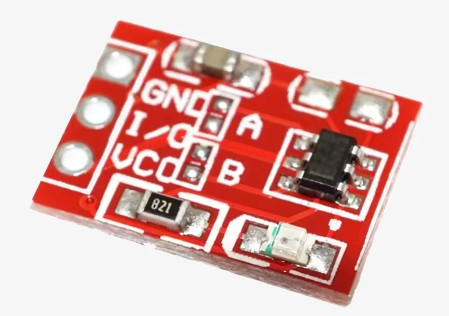
\includegraphics[width=\textwidth]{images/hardware/ttp223.jpg}
\captionof{figure}{TTP223 Capacitive Touch Sensor Module}
\label{fig:ttp223}
\end{minipage}
\hfill
\begin{minipage}{0.55\textwidth}
\textbf{Specifications:}
\begin{itemize}
    \item \textbf{Supply Voltage:} 2.4V–5.5V (nominally 3.3V or 5V)
    \item \textbf{Output:} Active-HIGH (1.8V–3.3V, depending on supply)
    \item \textbf{Sensitivity:} Adjustable via firmware
    \item \textbf{Response Time:} 60 ms typical
    \item \textbf{Detection Range:} ~5 mm through non-conductive materials
\end{itemize}
\end{minipage}

\vspace{0.4cm}
\noindent \textbf{Integration Notes:} TTP223 modules \textbf{must be powered from 3.3V, not 5V}, as overvoltage can damage GPIO inputs on the ESP32. Despite being rated for 5.5V operation, connecting a 5V-powered module to ESP32 GPIO creates an overvoltage risk.

\subsection{AHT10 Temperature and Humidity Sensor}

\noindent
\begin{minipage}{0.4\textwidth}
\centering
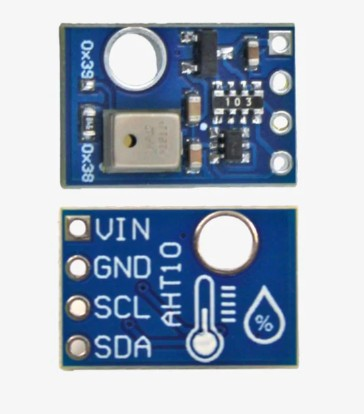
\includegraphics[width=\textwidth]{images/hardware/aht10.jpg}
\captionof{figure}{AHT10 Temperature/Humidity Sensor}
\label{fig:aht10}
\end{minipage}
\hfill
\begin{minipage}{0.55\textwidth}
\textbf{Specifications:}
\begin{itemize}
    \item \textbf{Supply Voltage:} 3.3V
    \item \textbf{Communication:} I2C (Address 0x38)
    \item \textbf{Temperature Range:} -40°C to +85°C (±2°C accuracy)
    \item \textbf{Humidity Range:} 0–100\% RH (±3\% accuracy)
    \item \textbf{Response Time:} 80 ms
    \item \textbf{Size:} Small DIP package, easy breadboarding
\end{itemize}
\end{minipage}

\vspace{0.4cm}
\noindent \textbf{Integration Notes:} The AHT10 communicates via I2C, sharing the same SDA/SCL lines with other sensors. Requires pull-up resistors (typically 4.7kΩ) on both lines.

\subsection{Status LEDs}

The system incorporates two light-emitting diodes (LEDs) to provide immediate visual feedback regarding the operating status of the device. A green LED, connected to GPIO 23, serves as the Wi-Fi connection indicator. When the device is successfully connected to the local wireless access point and authenticated with the Firebase Realtime Database, this LED remains solid green. During the pairing or connection process, it flashes at periodic intervals. A red LED, connected to GPIO 4, is used to indicate errors, connection drops, or initialization failures. Both LEDs are powered from the 3.3V logic rail and require 220\(\Omega\) current-limiting resistors in series to restrict the forward current and protect the ESP32 GPIO pins from overcurrent damage.

\subsection{Tactile Push Button (Mode/Pairing)}

A standard momentary tactile push button is connected to GPIO 0 to facilitate manual device provisioning and reset actions. In this circuit design, the switch is wired in an active-LOW configuration where one terminal is tied to the ESP32 input pin and the other is connected to common Ground. An internal pull-up resistor is enabled on GPIO 0 to hold the line at a logic HIGH state when the button is open. When pressed, the input is pulled to Ground (logic LOW), triggering an interrupt routine in the firmware. Since GPIO 0 is also an ESP32 strapping pin that controls the boot mode, the firmware is structured to ignore debounced signals during power-up to prevent the microcontroller from entering serial programming mode unintentionally.

\subsection{AC-DC Power Converter (5V, 2A SMPS)}

To power the entire smart switch system from standard household mains (220V AC, 50Hz), a compact AC-DC switched-mode power supply (SMPS) module is integrated. This step-down converter steps down the high-voltage AC mains to a regulated 5V DC output, capable of delivering up to 2A of continuous current. The 5V DC rail directly powers the 6-channel relay board, as the relay coils require a 5V supply to operate reliably. A portion of the 5V supply is routed through an onboard linear voltage regulator (AMS1117-3.3) to establish a stable 3.3V rail for the ESP32 DevKit, touch sensors, and the AHT10 sensor. A 2A rating is selected to prevent voltage sags when all six relays are energized simultaneously alongside peak WiFi transmission bursts from the ESP32.

\section{Circuit Design}

\begin{figure}[H]
\centering
\caption{NexusFlow Hardware Circuit Diagram}
\label{fig:circuit_diagram}
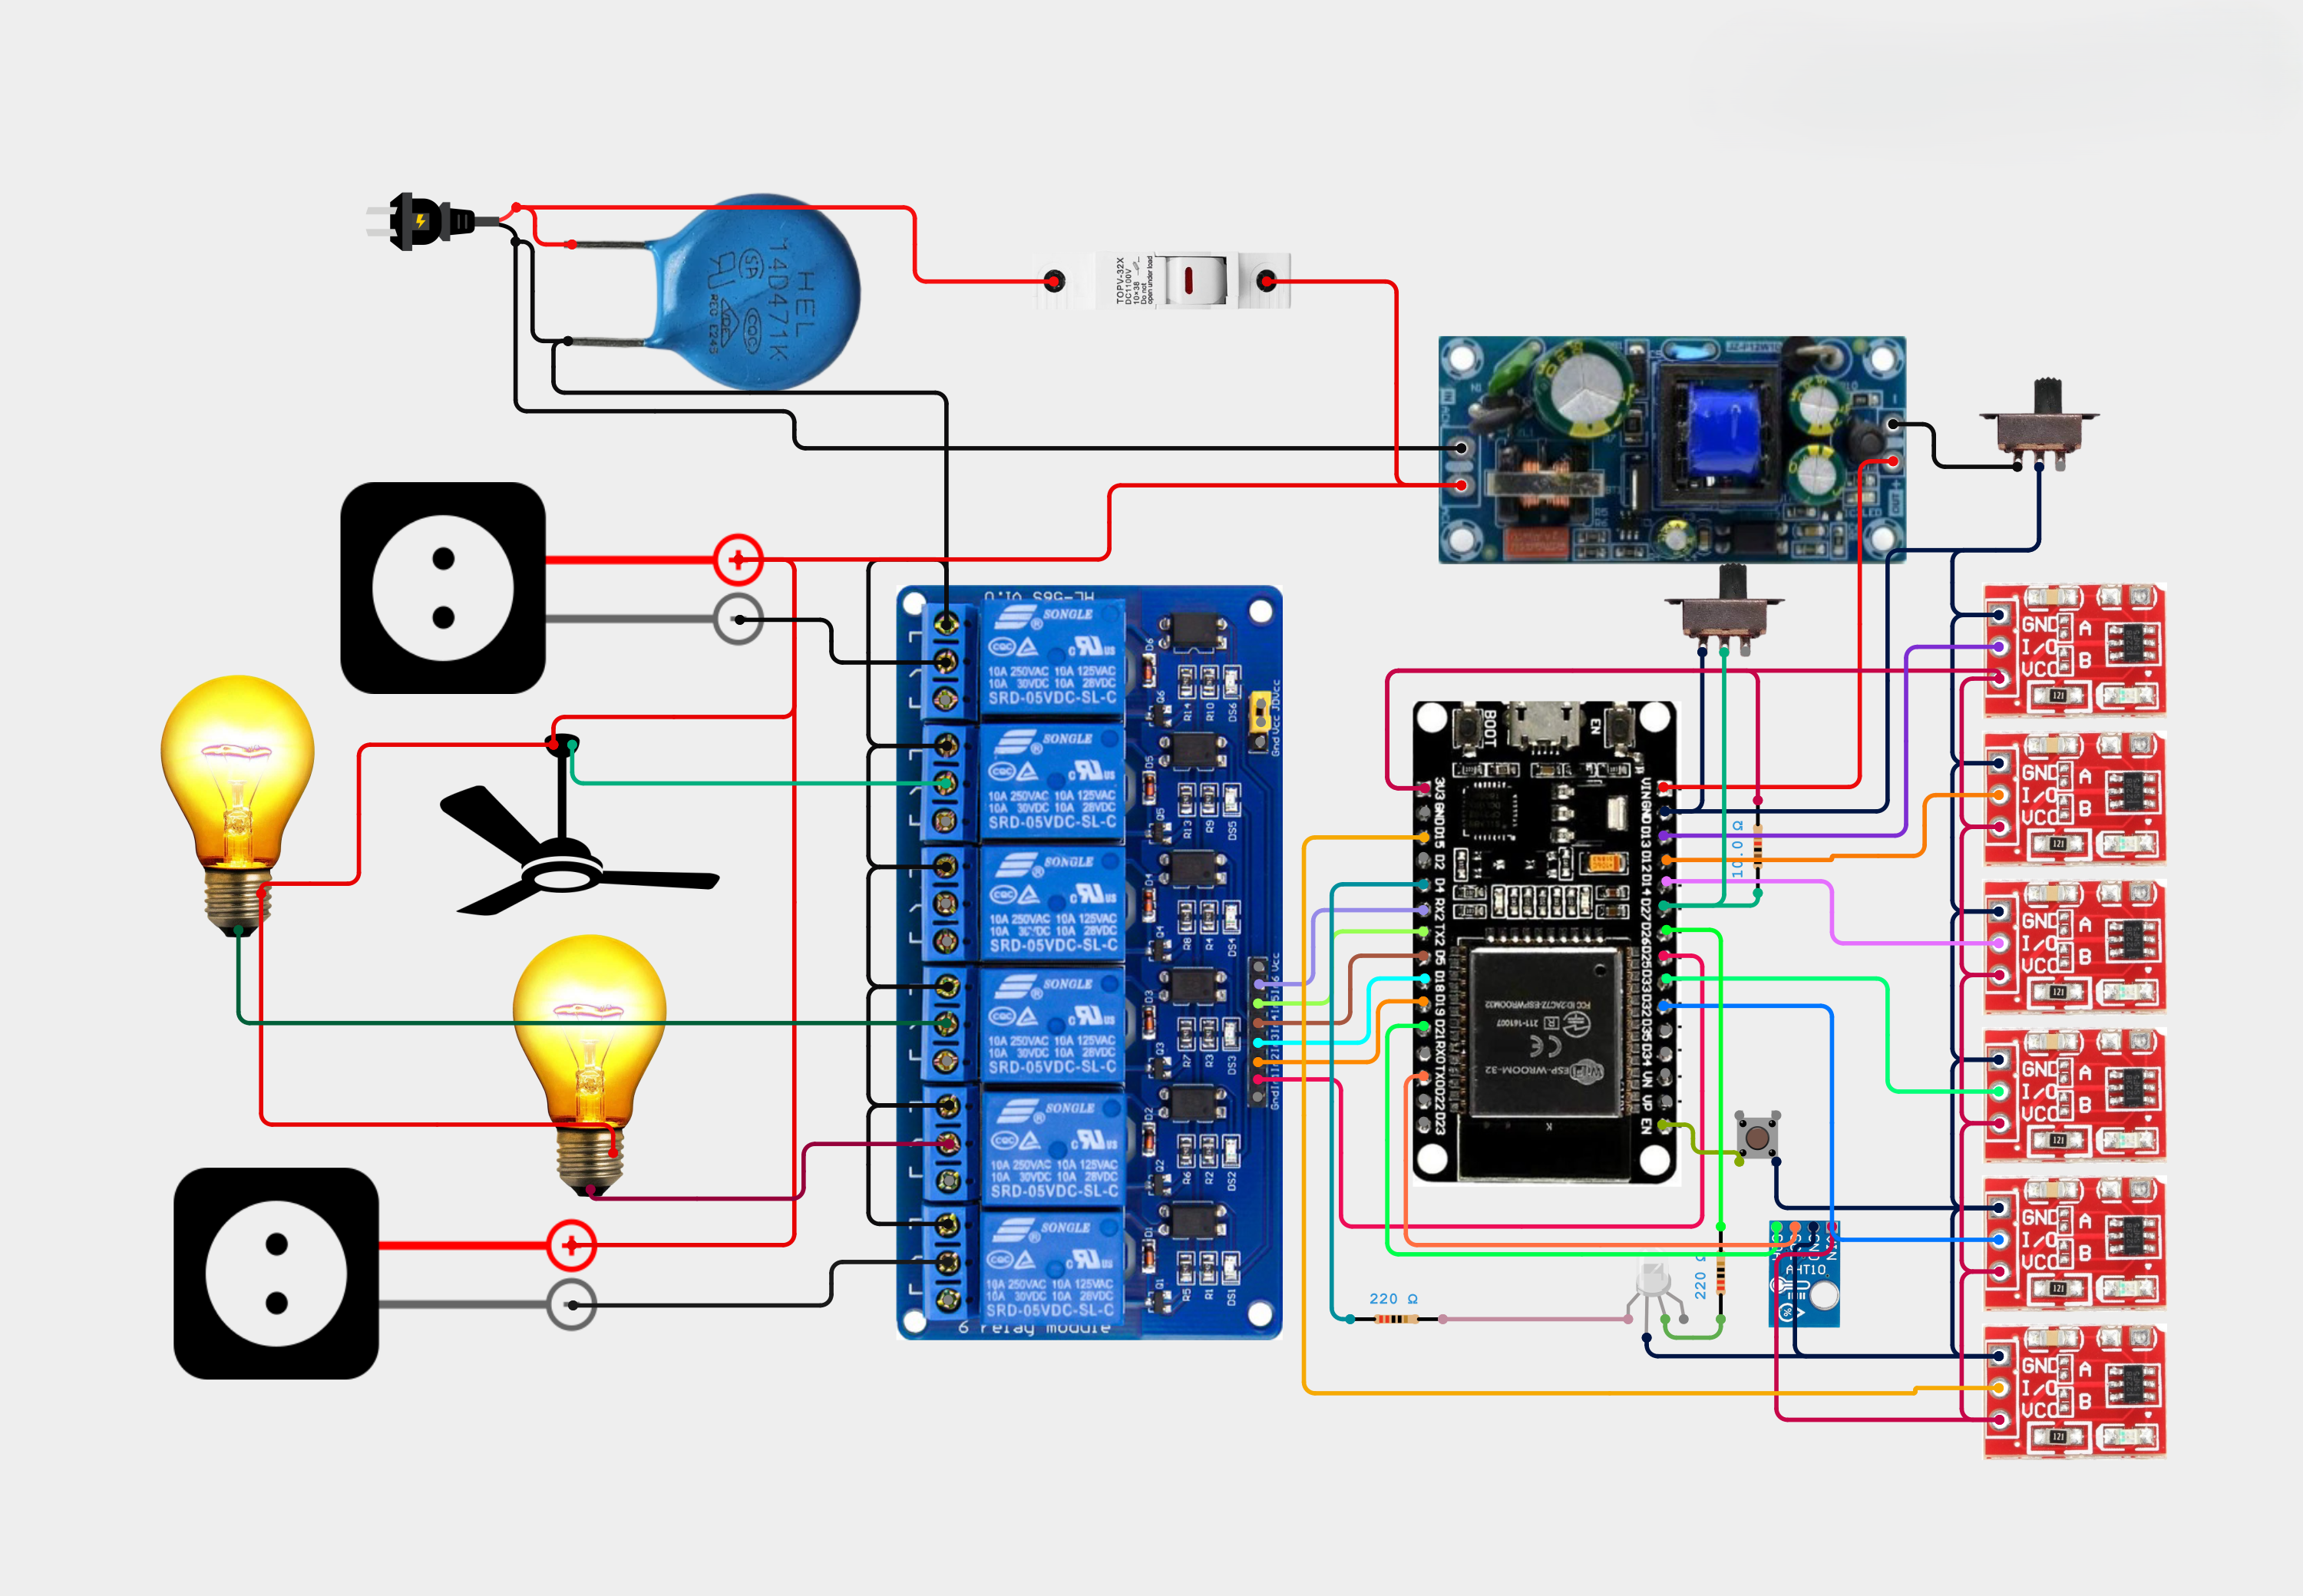
\includegraphics[width=0.75\textwidth]{images/hardware/circuit_diagram.png}
\end{figure}

\subsection{Power Distribution}

\begin{itemize}
    \item \textbf{5V Rail:} Supplies relay modules only
    \item \textbf{3.3V Rail:} Supplies ESP32, TTP223 modules, AHT10 sensor, status LEDs
    \item \textbf{Ground Plane:} Common ground for all components
\end{itemize}

All 3.3V connections include 0.1 µF bypass capacitors adjacent to component pins to suppress noise.

\subsection{Relay Control Circuit}

\begin{itemize}
    \item Each relay module IN pin connects to a dedicated ESP32 GPIO
    \item Relay modules are powered from 5V rail with common ground
    \item Relay switching contacts (NO/NC/COM) are isolated from logic circuits
    \item Protection diodes (1N4007) prevent backemf spikes
\end{itemize}

\subsection{Touch Sensor Input Circuit}

\begin{itemize}
    \item TTP223 OUT pins connect directly to ESP32 GPIO (3.3V tolerant)
    \item All TTP223 modules powered from 3.3V rail
    \item \textbf{Critical:} Never connect 5V relay module outputs to TTP223 VCC—overvoltage will damage the module and potentially the ESP32
\end{itemize}

\subsection{I2C Sensor Bus}

\begin{itemize}
    \item AHT10 SDA/SCL connect to ESP32 GPIO 21 (SDA) and 22 (SCL)
    \item 4.7 kΩ pull-up resistors on both lines to 3.3V
    \item 0.1 µF capacitors to ground on both lines for EMI filtering
\end{itemize}

\section{GPIO Pin Configuration}

\begin{table}[H]
\centering
\caption{ESP32 GPIO Pinout and Function Mapping}
\label{tbl:gpio_mapping}
\begin{tabular}{|c|c|c|c|}
\hline
\textbf{GPIO} & \textbf{Function} & \textbf{Mode} & \textbf{Notes} \\
\hline
0 & Mode/Pairing Button & INPUT (pull-up) & Strapping pin—boot behavior sensitive \\
\hline
4 & Red Status LED & OUTPUT & Error/Low battery indicator \\
\hline
5 & Relay 3 Control & OUTPUT & SPI CLK strapping pin (careful in boot) \\
\hline
12 & Touch Sensor 5 Input & INPUT & Strapping pin—boot behavior sensitive \\
\hline
13 & Touch Sensor 4 Input & INPUT & Standard GPIO \\
\hline
14 & Touch Sensor 3 Input & INPUT & Standard GPIO \\
\hline
15 & Touch Sensor 6 Input & INPUT & Strapping pin—output only during boot \\
\hline
16 & Relay 5 Control & OUTPUT & Standard GPIO \\
\hline
17 & Relay 4 Control & OUTPUT & Standard GPIO \\
\hline
18 & Relay 2 Control & OUTPUT & Standard GPIO \\
\hline
19 & Relay 1 Control & OUTPUT & Standard GPIO \\
\hline
21 & I2C SDA & I2C & Sensor communication \\
\hline
22 & I2C SCL & I2C & Sensor communication \\
\hline
23 & Green Status LED & OUTPUT & WiFi connection indicator \\
\hline
25 & Relay 6 Control & OUTPUT & Standard GPIO \\
\hline
27 & Mode-Select Slider & ANALOG INPUT & For mode selection logic \\
\hline
32 & Touch Sensor 1 Input & INPUT & Standard GPIO \\
\hline
33 & Touch Sensor 2 Input & INPUT & Standard GPIO \\
\hline
\end{tabular}
\end{table}

\subsection{Hardware Safety Callouts}

\subsubsection{Strapping Pins}

The ESP32 uses certain pins during boot to determine operating mode:

\begin{itemize}
    \item \textbf{GPIO 0:} If held LOW during power-up, device enters download/flash mode
    \item \textbf{GPIO 12:} If pulled HIGH during boot, incorrect voltage mode is selected
    \item \textbf{GPIO 15:} If held LOW during boot, SDIO mode is enabled
\end{itemize}

\textbf{Risk:} Using these pins as touch inputs with always-active buttons can interfere with normal boot. Mitigation: debounce firmware, ensure buttons don't engage during power-up, and include adequate pull-ups/pull-downs for predictable boot behavior.

\subsubsection{TTP223 Supply Voltage}

\textbf{Critical Warning:} TTP223 modules advertise 5.5V support but are extremely sensitive to overvoltage on logic outputs. Connecting a 5V-powered TTP223 module to ESP32 GPIO can cause:

\begin{itemize}
    \item GPIO overvoltage damage (GPIO max is 3.6V)
    \item Latch-up or device resets
    \item Unpredictable behavior or permanent damage
\end{itemize}

\textbf{Mitigation:} Always power TTP223 modules from 3.3V rail and verify output voltage is \(\leq\) 3.3V before connecting to ESP32.



\section{Bill of Materials (BOM)}

\begin{table}[H]
\centering
\caption{Hardware Component List (BOM)}
\label{tbl:bom}
\begin{tabular}{|l|c|c|c|}
\hline
\textbf{Component} & \textbf{Qty} & \textbf{Unit Cost (Rs.)} & \textbf{Total Cost (Rs.)} \\
\hline
ESP32 DevKit V1 & 1 & 380 & 380 \\
\hline
5V Relay Module (6-Channel) & 1 & 220 & 220 \\
\hline
TTP223 Capacitive Touch Module & 6 & 7 & 42 \\
\hline
AHT10 Temperature/Humidity Sensor & 1 & 85 & 85 \\
\hline
AC-DC Power Converter (5V, 2A SMPS) & 1 & 130 & 130 \\
\hline
Tactile Push Button (Mode/Pairing) & 1 & 5 & 5 \\
\hline
Status LEDs (Green/Red) & 2 & 2 & 4 \\
\hline
Resistors (220\(\Omega\), 4.7k\(\Omega\)) & 20 & 0.50 & 10 \\
\hline
Capacitors (0.1\(\mu\)F, 10\(\mu\)F) & 15 & 1.00 & 15 \\
\hline
Diodes (1N4007) & 6 & 1.00 & 6 \\
\hline
Perfboard / General Purpose PCB & 1 & 40 & 40 \\
\hline
USB Cable (for power/programming) & 1 & 50 & 50 \\
\hline
Jumper Wires (set) & 1 & 60 & 60 \\
\hline
\textbf{Total} &  &  & \textbf{1047} \\
\hline
\end{tabular}
\end{table}

\section{Assembly and Testing Checklist}

\subsection{Pre-Assembly}

\begin{itemize}
    \item [ ] Verify all components match datasheets
    \item [ ] Check for cold solder joints on module headers
    \item [ ] Inspect relay coils for visible damage
    \item [ ] Test ESP32 USB connectivity (recognizes as serial device)
\end{itemize}

\subsection{Assembly}

\begin{itemize}
    \item [ ] Mount ESP32 on breadboard/perfboard
    \item [ ] Connect 5V and 3.3V power rails with adequate decoupling capacitors
    \item [ ] Wire relay module IN pins to designated GPIO (see Table \ref{tbl:gpio_mapping})
    \item [ ] Wire TTP223 OUT pins to designated GPIO (ensure 3.3V supply)
    \item [ ] Connect AHT10 SDA/SCL to GPIO 21/22 with pull-up resistors
    \item [ ] Connect status LEDs with current-limiting resistors
    \item [ ] Connect mode button and mode-select slider
\end{itemize}

\subsection{Power-On Test}

\begin{itemize}
    \item [ ] Supply 5V power—ESP32 boot LED should illuminate
    \item [ ] Green status LED should blink (awaiting WiFi)
    \item [ ] No smoke or unusual heat from relay modules
    \item [ ] Touch each TTP223 input—verify corresponding GPIO triggers in serial monitor
\end{itemize}

\subsection{Functional Test}

\begin{itemize}
    \item [ ] Flash firmware—no errors during upload
    \item [ ] Serial monitor shows initialization messages
    \item [ ] BLE advertising begins after boot
    \item [ ] AHT10 sensor readings appear in logs
    \item [ ] Manual relay toggle via serial commands works
\end{itemize}

\section{Known Hardware Limitations}

\begin{itemize}
    \item \textbf{GPIO 12 / GPIO 15:} Strapping pins with non-zero boot sensitivity. Using them as touch inputs requires careful debouncing and may require board revision if unexpected resets occur.
    
    \item \textbf{I2C Pull-ups:} ESP32 has weak internal pull-ups. External 4.7kΩ resistors are recommended for reliable I2C communication, especially with multiple sensors.
    
    \item \textbf{USB Power Limitations:} Some USB cables or computer USB ports cannot reliably supply the current needed by ESP32 + 6 relays simultaneously. A powered USB hub or separate 5V supply is recommended for stable operation.
    
    \item \textbf{Relay Module Variability:} Different relay module clones have slightly different control logic (some active-HIGH, some active-LOW). Firmware must be verified against actual modules used.
\end{itemize}

\section{Future Hardware Improvements}

\begin{itemize}
    \item Custom PCB design to eliminate breadboard/perfboard fragility
    \item Isolated relay driver circuits to reduce EMI
    \item Battery backup (UPS) for maintaining automation during power outages
    \item Additional sensor support (motion detection, light level, air quality)
    \item Modular I/O expansion for channels beyond 8
\end{itemize}
